\section{Introduction}



\begin{figure*}
%\begin{tabular}{llp{2.2in}}
\begin{tabular}{llp{8in}}
send & recv & comments \\
wait & buf & \\
no & 1 & Messages dropped by sender. Observers are decoupled.\\
no & 2 & Messages dropped by sender or receiver.  Observers are decoupled. \\
no & 3 & Messages dropped by sender or receiver. Observers are decoupled. \\
post & 1 & No messages lost. Observers are coupled. \\
post & 2 & Messages dropped by receiver.  Observers are coupled.\\
post & 3 & Messages dropped by receiver.  Observers are coupled.\\
pre & 1 & No messages lost. Observers are coupled. \\
pre & 2 & Messages dropped by receiver. Observers are coupled.\\
pre & 3 & Messages dropped by receiver. Observers are coupled.
\end{tabular}

\end{figure*}


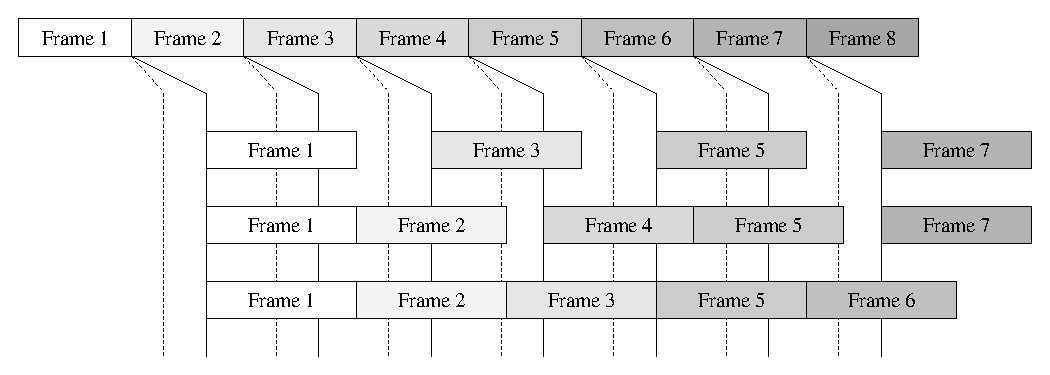
\includegraphics[width=\columnwidth]{fig-throughput-nowait}

\includegraphics[width=\columnwidth]{fig-throughput-prewait}

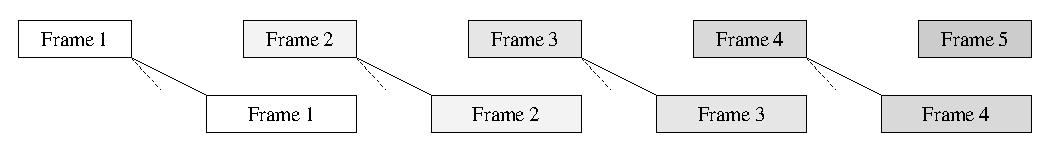
\includegraphics[width=\columnwidth]{fig-throughput-postwait}

Adaptive scheduling?  Could be difficult to reason about.


YARP is written by and for researchers in robotics, particularly
humanoid robotics, who find themselves with a complicated pile of
hardware to control with an equally complicated pile of software. 
%
At the time of writing (2005), running decent visual, auditory, and
tactile perception while performing elaborate motor control in
real-time requires a lot of computation. The easiest and most scalable
way to do this right now is to have a cluster of computers. Every year
what one machine can do grows, but so do our demands. YARP is a set of
tools we have found useful for meeting our computational needs for
controlling various humanoid robots.

\subsection*{Stopping the pain}

YARP is designed with robotics research groups in mind.  
%
%
It is targetted primarily at supporting software development.
%
%
Here are the assumptions we make, distilled from our own repeated
experience.  
%
%We express the assumptions in terms of {\em pain} --
%situations we would like to avoid.

\begin{itemize}

\item {\bf Humility is key.}
%
Over time, sofware for a sophisticated robot needs to 
aggregate code written by many different people in many
different contexts.  No doubt that code will have
dependencies on various communication, image processing,
and other libraries.
%
YARP needs to play well with these other libraries.
It should not try to ``take control'' of processes,
hardware management, or any kind of service.


\item {\bf Computing power should be scalable.}
%
Designing a robot control system as a set of processes running on
  a set of computers is a good way to work, especially if the robot
  is not mobile.  It minimizes time spent wrestling with code
  optimization, rewriting other people's code, etc., and maximizes
  time spent actually doing research.
  The heart of YARP is a communications mechanism to make writing
  and running such processes as easy as possible.


\item {\bf Never stop.}
%
The longer a process can stay running, the better.  Restarting
  processes often has a cost.  For example, it may talk to some
  custom hardware which requires a physical reset.  There may
  be other dependent processes that need to be restarted in turn.

  YARP does its part to minimize dependencies between processes.
  Communication channels between processes can come and go.
  A process that is killed or dies unexpectedly does not
  require processes to which it connects to be restarted



\end{itemize}


\subsection*{Zone of proximal development}

(this section is very vague)

For infants, the zone of proximal development is the
difference between what they can accomplish on their
own compared to what they can accompish with an
adult's support [CITE].

By loose analogy, we label a robot control system's ``zone of proximal
development'' to be the set of modules being actively added or worked
on by the programmer, against a background of pre-existing, operating
modules.  

YARP helps insulate existing modules from changes in this zone,
and leaves them in a good form for when the zone moves on.


\subsection*{Design patterns}

Communication in YARP follows the {\em Observer} pattern [CITE].  The state
of special {\tt Port} objects can be delivered to any number of
observers, in any number of processes distributed across any number of
machines.  The data source is isolated from management of the list
of observers.  Equally importantly, each observer is insulated as
much as possible from the effects of other observers.  For example,
if one observer reads a data source slowly and infrequently, this
does not doom other observers to slow operation.

(Maybe give an example from Cog? -- number of processes started up,
number of connections made...)

The fundamental image class in YARP can easily become a {\em Proxy}
to image data stored externally or in an alternate representation.

Our goal is that observers can be added to an observable without
having an impact on existing observers.  This has some important 
consequences:

\begin{itemize}

\item A ``slow'' observer, which takes time to process each update it
received from the observable, should not force a ``fast'' observer of
the same observable to slow down.  This implies either buffering
of messages for bursty channels, or simply dropping messages for
observers that can't keep up.  The second approach is the default
behavior in YARP.

\end{itemize}


On the sender side:

\begin{itemize}

\item Default behavior: every time an update is performed on an
observable, its state is made available to send to every
observer not currently still reading a previous state.

\item The programmer can optionally choose to wait until all observers
have finished reading and are in a ready state.

\end{itemize}

On the receiver side:

\begin{itemize}

\item Default (triple-buffer) behavior: an observer becomes free for
another update immediately after having received one, before any
processing is done at all.  If updates arrive faster than processing
occurs, then updates will be lost from time to time (where ``lost''
means ``never processed''), but the most recent update received will
always be read and available immediately when processing is completed.

\item Optional (double-buffer) behavior: same as above, but if an
update is currently arriving, then when processing completes no new
content will be available until the update arrives.  This is good if
it is better to minimize latency of non-dropped updates than to
maximize throughput.

\item Optional (single-buffer) behavior: the arrival of updates
is delayed until processing completes.  No updates will ever be 
thrown away on the receiver side.


\end{itemize}
